\documentclass[a4paper, 11pt]{article}
\usepackage[utf8]{inputenc}
\usepackage[T1]{fontenc}
\usepackage{amsmath, amsfonts, amssymb}
\usepackage{graphicx}
\usepackage{float}
\usepackage{hyperref}
\usepackage{enumitem}
\usepackage{booktabs}
\usepackage{longtable}
\usepackage{array}
\usepackage{multirow}
\usepackage{xcolor}
\usepackage{url}
\usepackage{fancyhdr}
\usepackage{textcomp}
\usepackage{arxiv}

% ── Avisos de datos preliminares ─────────────────────────────────────────────
% Para ocultar TODOS los avisos amarillos en la versión final, cambiar
% \mostraravisostrue por \mostraravisosfalse.
\newif\ifmostraravisos
\mostraravisostrue
\newcommand{\pendiente}{%
  \ifmostraravisos
    \par\medskip\noindent
    \colorbox{yellow}{\parbox{\dimexpr\linewidth-2\fboxsep\relax}{\small\textbf{[ESTOS DATOS SON ANTES DE TERMINAR EL PROYECTO, UNA VEZ TERMINADO VOLVER A ESCRIBIR ESTA CONCLUSIÓN/FOTO]}}}%
    \par\medskip
  \fi}

% ── Placeholders para links (AnyLogic Cloud, YouTube) ────────────────────────
% Reemplazar \completar{...} por \url{https://...} cuando estén los links.
\newcommand{\completar}[1]{%
  \par\medskip\noindent
  \fcolorbox{blue!60}{blue!8}{\parbox{\dimexpr\linewidth-2\fboxsep-2\fboxrule\relax}{\centering\small\textbf{[COMPLETAR: #1]}}}%
  \par\medskip}

% ── Columnas de tabla con texto ajustado ─────────────────────────────────────
\newcolumntype{L}[1]{>{\raggedright\arraybackslash}p{#1}}
\newcolumntype{C}[1]{>{\centering\arraybackslash}p{#1}}

% ── Header ────────────────────────────────────────────────────────────────────
\fancyhf{}
\rhead{\small TPI - SIMULACI\'ON DE EVACUACI\'ON EN AMERIZAJE - GRUPO 01 - COM. 402 - NOVIEMBRE 2026}
\rfoot{\thepage}
\renewcommand{\headrulewidth}{0pt}

% ── Rótulos en español ────────────────────────────────────────────────────────
\AtBeginDocument{%
  \renewcommand{\contentsname}{\'Indice}%
  \renewcommand{\figurename}{Figura}%
  \renewcommand{\tablename}{Tabla}%
  \renewcommand{\refname}{Referencias}%
  \renewcommand{\abstractname}{Resumen}%
}

\setlength{\parindent}{0pt}
\setlength{\parskip}{4pt}
\raggedbottom % evita que se estiren los espacios verticales cuando una figura/tabla no entra en la p\'agina

% ── Portada ───────────────────────────────────────────────────────────────────
\title{
    \vspace{-1cm}
    \begin{center}
        
\includegraphics[width=0.3\textwidth]{Image.jpg}
    \end{center}
    \rule{\linewidth}{0.5mm} \\[0.4cm]
    \textbf{\huge TPI - SIMULACI\'ON DE LA EVACUACI\'ON DE UN BOEING 737-800 EN UN AMERIZAJE} \\[0.4cm]
    \textbf{Asignatura:} Simulaci\'on \\
    \vspace{0.5cm}
    \normalsize Comisi\'on: 402 \quad $\cdot$ \quad Grupo: 01 \\[0.2cm]
    \rule{\linewidth}{0.5mm}
}

\author{
\textbf{Luis Parmigiani} \\
Legajo: 52933 \\
\textit{Universidad Tecnol\'ogica Nacional - FRRO} \\
Zeballos 1341, S2000, Argentina \\
\texttt{parmigianiluis04@gmail.com} \\[2mm]
\and
\textbf{Agust\'in Dana} \\
Legajo: 52935 \\
\textit{Universidad Tecnol\'ogica Nacional - FRRO} \\
Zeballos 1341, S2000, Argentina \\
\texttt{agusidana04@gmail.com} \\[2mm]
\and
\textbf{Bruno Vitali} \\
Legajo: 53137 \\
\textit{Universidad Tecnol\'ogica Nacional - FRRO} \\
Zeballos 1341, S2000, Argentina \\
\texttt{brunoVitali33@gmail.com} \\[2mm]
\and
\textbf{St\'efano Conti} \\
Legajo: 52850 \\
\textit{Universidad Tecnol\'ogica Nacional - FRRO} \\
Zeballos 1341, S2000, Argentina \\
\texttt{stefano.conti2004@gmail.com} \\[2mm]
}

% =============================================================================
\begin{document}
\maketitle

\begin{center}
    \normalsize \textbf{Profesores:} Juan Ignacio Torres (Pr\'actica) y
    Jorge Flamini (Teor\'ia) \\[0.3cm]
    \normalsize Noviembre 2026
\end{center}

% ── Índice ───────────────────────────────────────────────────────────────────
\newpage
\thispagestyle{empty}
\pagenumbering{roman}
\tableofcontents
\newpage
\pagenumbering{arabic}

% ── Abstract ──────────────────────────────────────────────────────────────────
\begin{abstract}
\noindent
El presente trabajo desarrolla un modelo de simulaci\'on basado en agentes,
implementado en AnyLogic con su Pedestrian Library, para estudiar la evacuaci\'on
de un Boeing 737-800 tras un amerizaje.
En lugar de reproducir el ensayo de certificaci\'on, el modelo somete al avi\'on a
condiciones m\'as cercanas a las de un evento real: equipaje de mano, pasajeros con
movilidad reducida, iluminaci\'on de emergencia, salidas que deben abrirse y cuya
disponibilidad los pasajeros desconocen, y una tripulaci\'on que evac\'ua en
\'ultimo lugar.
Sobre la cabina modelada (186 pasajeros y 6 tripulantes, con las salidas traseras
inutilizables por la actitud de cola baja del amerizaje) se evaluaron cuatro
escenarios de disponibilidad de salidas y un an\'alisis de sensibilidad de 0 a 5
salidas bloqueadas, con 30 r\'eplicas por configuraci\'on.
Ninguna de las 300 corridas evacu\'o a los 192 ocupantes dentro del umbral de
90~segundos que fija la norma 14 CFR 25.803: aun con todas las salidas utilizables
disponibles, el tiempo mediano fue de 223,4~s.
El modelo reproduce cualitativamente los patrones de evacuaci\'on documentados en
el amerizaje del vuelo 1549 de US Airways en el r\'io Hudson.
Los resultados se proponen como insumo para que los organismos certificadores
eval\'uen si el umbral de 90~segundos sigue siendo representativo bajo condiciones
m\'as realistas.
\end{abstract}

\vspace{0.5cm}
\noindent\textbf{Palabras clave:} Simulaci\'on $\cdot$ Simulaci\'on basada en agentes
$\cdot$ AnyLogic $\cdot$ Pedestrian Library $\cdot$ Evacuaci\'on de emergencia
$\cdot$ Amerizaje $\cdot$ Boeing 737-800 $\cdot$ 14 CFR 25.803
$\cdot$ Regla de los 90 segundos $\cdot$ Vuelo 1549

% =============================================================================
\newpage
\section{Introducci\'on}
% =============================================================================

Este trabajo pr\'actico integrador propone el desarrollo de un modelo de
simulaci\'on basado en agentes para estudiar la evacuaci\'on de pasajeros en un
escenario de amerizaje (\textit{ditching}) de una aeronave comercial. El objetivo
general es evaluar, mediante simulaci\'on en AnyLogic y su Pedestrian Library, si
distintas configuraciones de salidas disponibles y condiciones realistas de cabina
permiten cumplir con el est\'andar regulatorio de evacuaci\'on en 90 segundos que
introduce la norma 14 CFR 25.803(c)\footnote{\textit{Emergency evacuation} de la
Federal Aviation Administration (FAA) de Estados Unidos (con su equivalente europeo
en la normativa EASA CS-25.803)~\cite{cfr25803}.}, o si bajo ciertas combinaciones
de factores ese umbral deja de ser alcanzable.

En una primera instancia, el trabajo se plante\'o como una verificaci\'on:
comprobar si el Boeing 737-800 cumple efectivamente con el umbral de 90 segundos.
A medida que avanz\'o la construcci\'on del modelo, el equipo concluy\'o que el
aporte de mayor valor no era reproducir la demostraci\'on de certificaci\'on, sino
someter al avi\'on a condiciones m\'as cercanas a las de un evento real que las del
ensayo normativo: pasajeros con equipaje de mano y con movilidad reducida, salidas
que deben abrirse y cuya disponibilidad los pasajeros desconocen, iluminaci\'on de
emergencia y una tripulaci\'on que evac\'ua en \'ultimo lugar. \textbf{Sobre esa base,
el objetivo pas\'o a ser analizar si, bajo estas condiciones, el umbral de 90
segundos sigue siendo un par\'ametro representativo o si deber\'ia revisarse.}

Si bien la certificaci\'on de amerizaje concretamente (14 CFR
25.801)~\cite{cfr25801} valida el comportamiento estructural e hidrodin\'amico del
avi\'on en el agua y no establece por s\'i misma un tiempo de evacuaci\'on, es la
norma 14 CFR 25.803 la que efectivamente fija el umbral de 90 segundos contra el
cual se eval\'uan los resultados de este trabajo, independientemente del tipo de
emergencia.

Para eso, se construye un modelo de la cabina de un Boeing 737-800 con su
disposici\'on real de salidas y pasillo, poblado por pasajeros, agentes con
atributos heterog\'eneos de movilidad, edad y comportamiento, calibrados a partir de
literatura acad\'emica\footnote{\textit{Emergency evacuation simulation of
commercial aircraft}, publicado en SN Applied Sciences (Springer,
2021)~\cite{gobbin2021}. Los par\'ametros de velocidad de caminata, dimensiones
corporales y comportamiento de conflicto se encuentran en la secci\'on de
resultados y discusi\'on del modelo.} sobre egreso de cabina. Sobre ese modelo se
comparan m\'ultiples escenarios, desde el caso ideal con todas las salidas
operativas hasta configuraciones de bloqueo parcial o asim\'etrico, bajo un
conjunto fijo de condiciones de piso realista (obst\'aculos, iluminaci\'on
reducida, ausencia de aviso previo). Los resultados se contrastan tanto contra el
est\'andar normativo de certificaci\'on como contra un caso real documentado de
amerizaje exitoso, para evaluar la representatividad del modelo y extraer
conclusiones sobre los factores que m\'as inciden en el tiempo de evacuaci\'on.

% =============================================================================
\newpage
\section{El problema}
% =============================================================================

\subsection{Marco regulatorio}\label{sub:marco}

La certificaci\'on de aeronavegabilidad exige que la cabina de pasajeros pueda
evacuarse completamente en 90 segundos, usando solo la mitad de las salidas de
emergencia disponibles (supuesto pensado para representar un escenario donde parte
de las salidas queda inutilizable tras una emergencia como ser\'ia, en nuestro caso
de estudio, un aterrizaje forzoso en el agua). Esta demostraci\'on se realiza bajo
condiciones deliberadamente adversas: de noche o con oscuridad simulada, usando
exclusivamente el sistema de iluminaci\'on de emergencia, y sin aviso previo a los
pasajeros sobre cu\'ales ser\'an las salidas bloqueadas\footnote{Este factor es
desconocido por la naturaleza del incidente, que hasta que no ocurra o no se
proceda a tratar de abrir dichas salidas no se sabe con certeza qu\'e salidas
quedar\'an bloqueadas.}.

Sin embargo, existe un cuestionamiento creciente sobre si estas condiciones de
ensayo siguen representando un escenario realista. Publicaciones especializadas del
sector aeron\'autico~\cite{raes_gone90} se\~nalan que factores como las dimensiones
de los asientos, la cantidad de equipaje de mano que llevan los pasajeros hoy y la
tendencia de los pasajeros a detenerse a recuperar equipaje de mano durante una
evacuaci\'on real no se han actualizado al mismo ritmo que la norma o no se han
tenido en cuenta en la misma, lo que abre la pregunta de si el est\'andar de 90
segundos sigue siendo un umbral representativo.

\subsection{Caso real}

El 15 de enero de 2009, poco despu\'es de despegar del aeropuerto LaGuardia con
destino a Charlotte, el Airbus A320-214 que operaba el vuelo 1549 de US Airways
impact\'o contra una bandada de gansos canadienses a unos dos minutos de vuelo, lo
que provoc\'o una p\'erdida casi total de empuje en ambos motores. Dada la altitud
y la posici\'on del avi\'on respecto a los aeropuertos cercanos, el capit\'an
Chesley ``Sully'' Sullenberger y el primer oficial Jeffrey Skiles determinaron que
no era viable intentar un regreso a LaGuardia ni un desv\'io a Teterboro, por lo
que decidieron planear el avi\'on hasta amerizar en el r\'io Hudson, cerca de
Midtown Manhattan. El amerizaje ocurri\'o menos de cuatro minutos despu\'es del
impacto con las aves, sin da\~nos estructurales significativos en el momento del
contacto con el agua, y los 155 ocupantes sobrevivieron~\cite{wiki1549}.

El caso del vuelo 1549 de US Airways (el amerizaje en el r\'io Hudson en enero de
2009) ofrece evidencia concreta de esta brecha entre lo que asume la
certificaci\'on y lo que ocurre en un evento real. Los 150 pasajeros y 5
tripulantes evacuaron por las salidas delanteras y sobre el ala, ya que las salidas
traseras no resultaron utilizables tras el amerizaje\footnote{Ya que el impacto
contra el agua da\~n\'o estructuralmente la secci\'on trasera del fuselaje,
provocando el ingreso de agua hacia esa parte de la cabina e inutilizando las dos
salidas traseras.}.

El avi\'on involucrado en el caso Hudson fue un Airbus A320-214, de la misma
categor\'ia (\textit{narrowbody}, un solo pasillo) que el Boeing 737-800 elegido
para este trabajo, aunque de fabricante y modelo distintos. Cabe destacar que dicho
vuelo no operaba bajo el r\'egimen regulatorio EOW (\textit{Extended Operations over
Water}) que exige provisiones de amerizaje\footnote{Informe NTSB/AAR-10/03,
secci\'on 1.5.3: ``Title 14 CFR 1.1, \textit{General Definitions}''~\cite{ntsb2010}.}
aunque igualmente llevaba el equipamiento de amerizaje instalado
(toboganes/balsas), por lo que evacu\'o exitosamente sin estar formalmente obligado
a cumplir con esa certificaci\'on espec\'ifica. El Boeing 737-800 s\'i cuenta con la
certificaci\'on opcional de amerizaje (\textit{Ditching Provisions}, 14 CFR 25.801),
seg\'un su \textit{Type Certificate Data Sheet}~\cite{easa_tcds737}.

De los 155 ocupantes, una minor\'ia fue rescatada a trav\'es de los
toboganes/balsas de las puertas delanteras, mientras que la mayor\'ia evacu\'o por
las salidas sobre el ala hacia las alas del avi\'on (un patr\'on de uso de salidas
notablemente distinto al que suele asumirse en un ensayo de certificaci\'on
sim\'etrico). Adem\'as, la certificaci\'on de aeronavegabilidad espec\'ifica para
amerizaje es opcional y no se exige a todos los aviones de transporte, lo que ha
llevado a cuestionamientos sobre qu\'e tan rigurosamente se validan en la pr\'actica
los supuestos de evacuaci\'on en agua.

\subsection{Planteamiento del problema}

Esta combinaci\'on (una norma que fija un umbral fijo bajo condiciones
estandarizadas, cuestionamientos documentados sobre su realismo, y al menos un caso
real donde el patr\'on de evacuaci\'on difiri\'o del supuesto por defecto) plantea
la pregunta central de este trabajo: \textbf{¿en qu\'e medida el cumplimiento de la
regla de los 90 segundos se sostiene bajo distintas configuraciones de salidas
disponibles y condiciones de piso realistas, m\'as all\'a del escenario
estandarizado de certificaci\'on?}

Dado que esta certificaci\'on espec\'ifica, como ya se mencion\'o anteriormente, no
es obligatoria para todos los aviones de transporte, y que los criterios sobre los
que se aprueba no siempre son sometidos a un escrutinio riguroso (como evidenci\'o
el propio NTSB al cuestionar los supuestos presentados en la certificaci\'on de
amerizaje del avi\'on del caso Hudson\footnote{Presentes en la secci\'on 1.6.7 del
informe NTSB~\cite{ntsb2010}.}), consideramos pertinente desarrollar un modelo que
no se limite a reproducir el ensayo de certificaci\'on, sino que incorpore
condiciones de cabina m\'as cercanas a las de un evento real. El objetivo no es
determinar si el Boeing 737-800 aprueba o no la certificaci\'on vigente, sino
aportar evidencia sobre cu\'anto se aleja el tiempo de evacuaci\'on del umbral de 90
segundos cuando las condiciones dejan de ser las estandarizadas. \textbf{De esta
forma, los organismos certificadores podr\'ian evaluar la validez de este escenario
m\'as realista y decidir si corresponde mantener el umbral, ampliarlo o exigir que
las aeronaves vuelvan a demostrar su cumplimiento bajo condiciones m\'as exigentes.}

% =============================================================================
\newpage
\section{Objetivos}\label{sec:objetivos}
% =============================================================================

\textbf{Objetivo general.} Evaluar, mediante un modelo de simulaci\'on basado en
agentes, si el umbral de evacuaci\'on de 90 segundos de la norma 14 CFR
25.803~\cite{cfr25803} sigue siendo representativo cuando la evacuaci\'on de un
Boeing 737-800 tras un amerizaje se somete a condiciones m\'as cercanas a las de un
evento real.

\textbf{Objetivos espec\'ificos.}
\begin{enumerate}[leftmargin=2em]
    \item Construir en AnyLogic un modelo de la cabina del Boeing 737-800 con su
          disposici\'on real de asientos, pasillo y salidas, poblado por agentes
          heterog\'eneos calibrados a partir de la literatura y de los requisitos del
          Appendix J~\cite{cfrAppJ}.
    \item Cuantificar el tiempo total de evacuaci\'on en cuatro configuraciones de
          salidas disponibles, con 30 r\'eplicas por configuraci\'on.
    \item Analizar la sensibilidad del tiempo de evacuaci\'on a la cantidad de
          salidas bloqueadas.
    \item Identificar los factores y cuellos de botella que m\'as inciden en el
          tiempo de evacuaci\'on.
    \item Validar cualitativamente el comportamiento del modelo contra la
          evacuaci\'on documentada del vuelo 1549 de US Airways.
    \item Aportar evidencia para que los organismos certificadores eval\'uen la
          vigencia del umbral bajo condiciones m\'as realistas.
\end{enumerate}

% =============================================================================
\newpage
\section{Metodolog\'ia}\label{sec:metodologia}
% =============================================================================

La metodolog\'ia se organiza en tres etapas: el dise\~no de los experimentos a
partir del problema planteado, la construcci\'on del modelo computacional en
AnyLogic y su verificaci\'on y validaci\'on antes de ejecutar las corridas cuyos
resultados se presentan en la secci\'on~\ref{sec:resultados}.

\subsection{Dise\~no de experimentos}\label{sec:diseno}

\subsubsection{Ajuste al universo de salidas disponibles}\label{sub:ajuste}

Antes de definir la matriz de escenarios, se incorpora una condici\'on estructural
fija: durante un amerizaje, la t\'ecnica est\'andar de aproximaci\'on exige una
actitud de morro (cabina) elevado (10\textdegree--12\textdegree) sobre la l\'inea de
flotaci\'on, lo que provoca que la secci\'on trasera del fuselaje reciba el primer y
m\'as severo impacto contra el agua. Este fen\'omeno, documentado tanto en estudios
de din\'amica de fluidos como en casos reales de amerizaje en distintos modelos de
avi\'on, tiene dos consecuencias que afectan directamente a las salidas traseras:
(a)~el da\~no estructural concentrado en esa zona, y (b)~la actitud de flotaci\'on
resultante (``cola hundida''), que sumerge las puertas traseras bajo la l\'inea de
flotaci\'on. Por este motivo, las dos salidas traseras (puertas 2L/2R) del Boeing
737-800 se consideran \textbf{inutilizables en todos los escenarios del modelo},
como condici\'on fija y no forman parte del universo de salidas disponibles.

En consecuencia, el universo de salidas sobre el que se construye la matriz de
escenarios queda reducido de 8 a \textbf{6 salidas}: el par delantero
(1L/1R\footnote{L proviene de la palabra \textit{``left''} del ingl\'es y R de la
palabra \textit{``right''}, que significan izquierda y derecha respectivamente.},
tipo~I\footnote{Seg\'un la clasificaci\'on oficial del 25.807 \textit{``Emergency
exits''}~\cite{cfr25807}.}) y los dos pares sobre el ala (tipo~III). Esta
redefinici\'on, adem\'as, acerca el modelo a lo observado en el caso real del vuelo
1549, donde la evacuaci\'on se realiz\'o exclusivamente por salidas delanteras y
sobre el ala.

\begin{figure}[H]
    \centering
    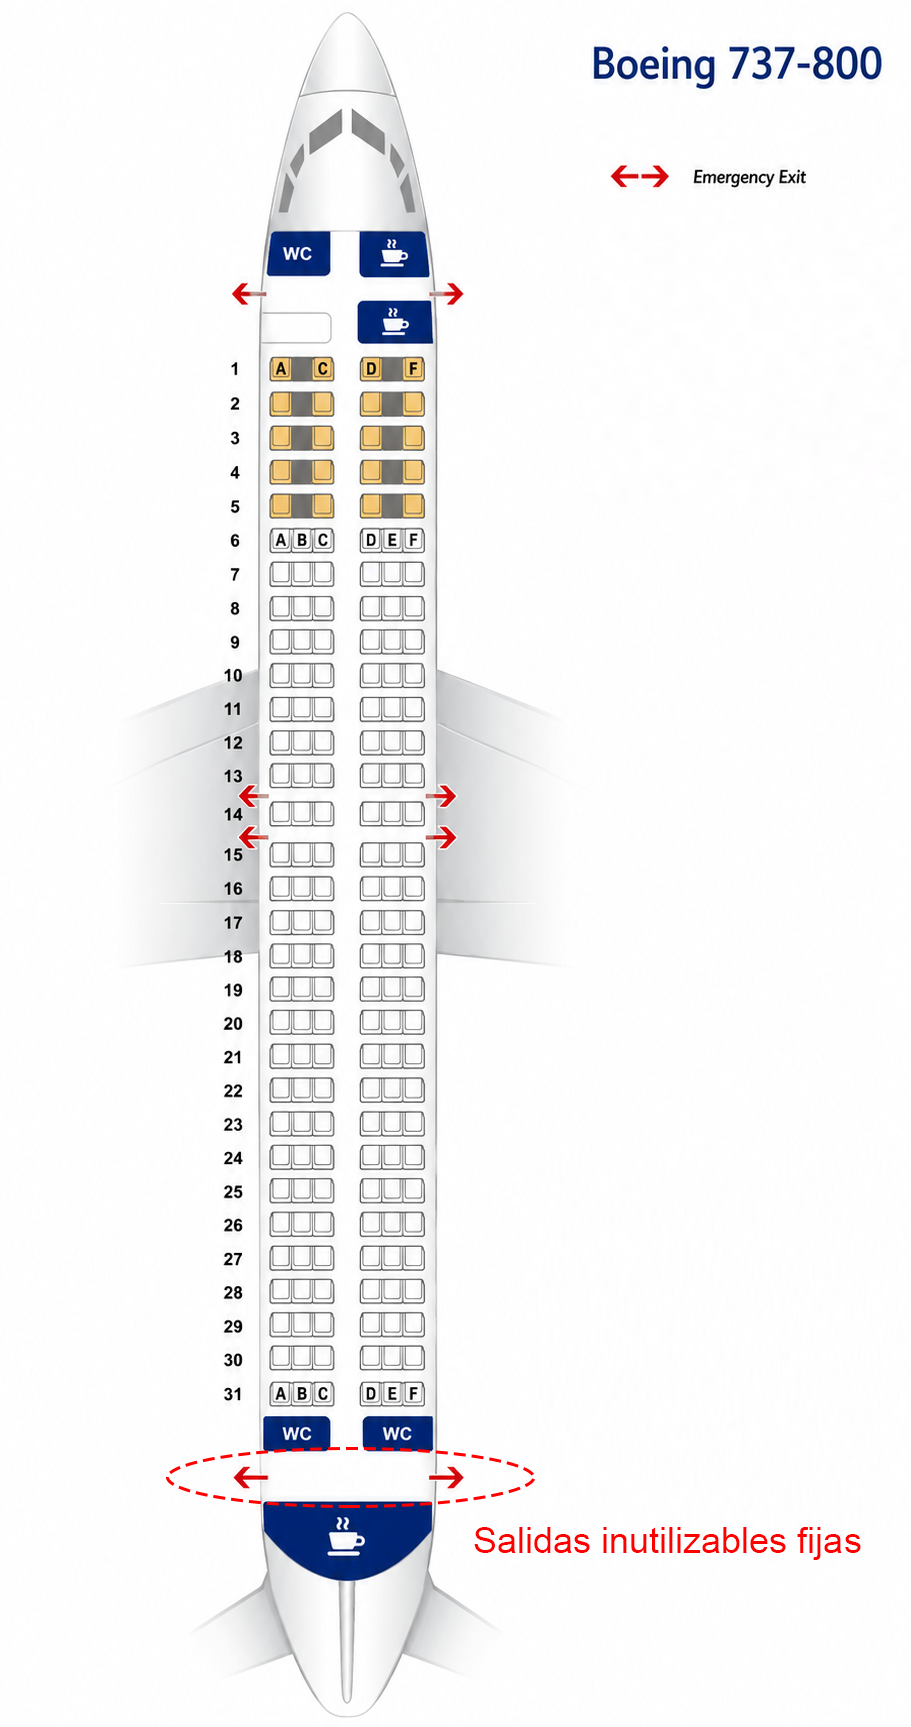
\includegraphics[width=0.42\textwidth]{fig1_salidas.png}
    \caption{Disposici\'on de salidas del Boeing 737-800 considerada en el modelo:
    en rojo, las dos salidas traseras (2L/2R), inutilizables en todos los
    escenarios por la actitud de cola baja caracter\'istica del amerizaje; las
    flechas rojas sin marcar, las 6 salidas restantes que conforman el universo
    variable sobre el que se construyen los escenarios.}
    \label{fig:salidas}
\end{figure}

\subsubsection{Matriz de escenarios}\label{sub:matriz}

\begin{table}[H]
\centering
\small
\begin{tabular}{C{1.3cm}L{3.4cm}L{4.6cm}L{4.6cm}}
\toprule
\textbf{N\'umero} & \textbf{Escenario} & \textbf{Salidas activas} & \textbf{Salidas bloqueadas} \\
\midrule
1 & Baseline & Las 6 (delanteras + 4 sobre el ala) & Ninguna (adem\'as de las traseras, ya fijas) \\
\midrule
2 & 50\% bloqueado, alternado (tipo certificaci\'on) & 3 de 6, alternadas entre ambos lados (ej.\ 1L, ala derecha delantera, ala izquierda trasera) & 3 de 6, distribuidas para no concentrar el bloqueo en un solo lado \\
\midrule
3 & 50\% bloqueado (libre el centro) & 3 de 6, concentradas en las salidas centrales sobre el ala & Las 3 restantes \\
\midrule
4 & Bloqueo asim\'etrico (un lado completo) & Solo las 3 salidas de un lado (1 delantera + 2 sobre el ala) & Las 3 salidas del lado contrario \\
\bottomrule
\end{tabular}
\caption{Matriz de escenarios.}
\label{tab:escenarios}
\end{table}

\subsubsection{Condiciones fijas}\label{sub:fijas}

Se agrega a las condiciones ya definidas (obst\'aculo en el pasillo, iluminaci\'on
reducida, ausencia de aviso previo, menor cantidad de tripulantes-gu\'ia):

\begin{itemize}[leftmargin=2em]
    \item Salidas traseras (2L/2R) inutilizables en todos los escenarios, por la
          raz\'on estructural/hidrodin\'amica explicada en la secci\'on~\ref{sub:ajuste}.
\end{itemize}

\subsubsection{M\'etricas a registrar}\label{sub:metricas}

Para cada uno de los 4 escenarios se ejecutan 30 corridas independientes en
AnyLogic (\textit{Parameter Variation} / \textit{Multi-run}), dado el componente
estoc\'astico en la velocidad y el comportamiento de los agentes. Se registra:

\textbf{Por corrida individual:}
\begin{itemize}[leftmargin=2em]
    \item Tiempo total de evacuaci\'on (desde el amerizaje hasta que sale el
          \'ultimo ocupante, tripulaci\'on inclu\'ida conforme a la regla).
    \item Tiempo de evacuaci\'on de pasajeros (hasta que sale el \'ultimo pasajero.
          Se registra como m\'etrica complementaria, para poder separar cu\'anto del
          tiempo total corresponde a la salida de la tripulaci\'on).
    \item Tiempo de salida del \'ultimo agente por cada una de las 6 salidas activas.
    \item Cantidad de pasajeros evacuados por cada salida (\textit{throughput} por
          salida).
    \item Tiempo individual de evacuaci\'on de cada agente (para poder construir
          distribuciones, no solo promedios).
    \item Cumplimiento o no del umbral de 90 segundos (variable binaria por corrida).
\end{itemize}

\textbf{Agregadas por escenario, tras las 30 corridas:}
\begin{itemize}[leftmargin=2em]
    \item Media y desv\'io est\'andar del tiempo total de evacuaci\'on.
    \item Percentil 95 (el peor 5\% de los casos), como medida de margen de seguridad
          m\'as exigente que el promedio.
    \item Porcentaje de corridas que efectivamente cumplen los 90 segundos.
    \item Salida con mayor \textit{throughput} y salida con mayor tiempo de
          saturaci\'on, por escenario (para identificar cuellos de botella
          recurrentes).
\end{itemize}

Los resultados de cada corrida individual se exportan a CSV/Excel para luego
calcular las m\'etricas por escenario, comparar contra el umbral de 90 segundos, e
identificar cuellos de botella recurrentes (como mencionamos en el p\'arrafo
previo).

\subsubsection{Gr\'aficos}\label{sub:graficos}

\begin{itemize}[leftmargin=2em]
    \item \textbf{Barras con intervalo de confianza:} tiempo medio de evacuaci\'on
          por escenario, con una l\'inea horizontal marcando el umbral de 90
          segundos, para ver de un vistazo qu\'e escenarios cumplen y cu\'ales no.
    \item \textbf{Boxplot por escenario:} distribuci\'on completa de los tiempos de
          evacuaci\'on (las 30 corridas), para mostrar dispersi\'on y valores
          at\'ipicos, no solo el promedio.
    \item \textbf{Curva de sensibilidad:} tiempo de evacuaci\'on vs.\ porcentaje de
          salidas bloqueadas, para mostrar la tendencia general de degradaci\'on a
          medida que se pierden salidas.
    \item \textbf{Curva de evacuaci\'on acumulada:} pasajeros evacuados acumulados en
          funci\'on del tiempo, una curva por escenario superpuestas en el mismo
          gr\'afico (es el gr\'afico cl\'asico de estudios de egreso, y permite
          comparar visualmente la velocidad de evacuaci\'on de cada configuraci\'on,
          no solo el tiempo final).
    \item \textbf{Throughput por salida:} barras apiladas o agrupadas mostrando
          cu\'antos pasajeros us\'o cada salida en cada escenario, para visualizar
          d\'onde se concentra la congesti\'on.
\end{itemize}

% =============================================================================
\newpage
\subsection{Construcci\'on del modelo en AnyLogic}\label{sec:construccion}
% =============================================================================

\subsubsection{Modelo conceptual}\label{sub:conceptual}

Antes de implementar el modelo en AnyLogic se defini\'o su estructura conceptual:
las entidades que intervienen en la evacuaci\'on, sus atributos, los eventos que
modifican el estado del sistema y los estados por los que atraviesa cada ocupante.
La Tabla~\ref{tab:conceptual} resume esa estructura; las subsecciones siguientes
detallan c\'omo se implement\'o cada elemento.

\begin{table}[H]
\centering
\small
\begin{tabular}{L{2.6cm} L{11.4cm}}
\toprule
\textbf{Elemento} & \textbf{Descripci\'on} \\
\midrule
Entidades & Pasajeros (186), tripulantes (6), salidas de emergencia y
obst\'aculos en el pasillo. \\
Atributos del pasajero & Sexo y franja etaria, velocidad preferida, movilidad
reducida, equipaje de mano, menor a cargo, asiento asignado y salida elegida. \\
Atributos de la salida & Tipo (I o III), ubicaci\'on, tiempo de apertura y estado
(activa o bloqueada seg\'un el escenario). \\
Eventos & Amerizaje ($t=0$, se\~nal de evacuaci\'on), apertura de cada salida,
llegada de un ocupante a la salida, egreso de cada ocupante y egreso del \'ultimo
ocupante (fin de la corrida). \\
Estados del ocupante & Sentado $\rightarrow$ saliendo de la fila $\rightarrow$
recorriendo el pasillo $\rightarrow$ esperando en la salida $\rightarrow$
evacuado. \\
Variables de respuesta & Tiempo total de evacuaci\'on, tiempo del \'ultimo
pasajero, ocupantes evacuados a los 90~s y uso de cada salida. \\
\bottomrule
\end{tabular}
\caption{Modelo conceptual del sistema simulado.}
\label{tab:conceptual}
\end{table}

\subsubsection{Entorno y geometr\'ia de la cabina}\label{sub:entorno}

Para la construcci\'on f\'isica del modelo se utiliz\'o como referencia una
fotograf\'ia de la distribuci\'on de asientos del Boeing 737-800 que, a diferencia
de la mayor\'ia de los planos comerciales disponibles para elecci\'on de asientos,
incluye la ubicaci\'on de las salidas de emergencia centrales. Estas salidas tienen
forma de ventana y son los propios pasajeros contiguos quienes las abren, previa
instrucci\'on de la tripulaci\'on de cabina.

Previo al aterrizaje de emergencia, todos los pasajeros y los 4 tripulantes de
cabina se encuentran en sus asientos. Al momento del impacto, la tripulaci\'on se
divide en dos grupos: dos tripulantes permanecen en la parte delantera del avi\'on
(antes de la cabina de mando) y dos en la parte trasera. Cuando el piloto comunica
la decisi\'on de realizar un aterrizaje de emergencia, la tripulaci\'on de cabina
instruye a los pasajeros contiguos a las salidas de emergencia centrales sobre
c\'omo abrirlas una vez producido el impacto.

Como se detall\'o en la secci\'on~\ref{sub:ajuste}, si bien el avi\'on cuenta con 8 salidas de
emergencia, solo 6 resultan utilizables en un escenario de amerizaje, dado que el
dise\~no del avi\'on lo hace flotar con la cola hundida, inutilizando las dos
salidas traseras. En consecuencia, los dos tripulantes de la parte trasera cumplen
la funci\'on de guiar a los pasajeros de esa zona hacia las salidas delanteras, por
lo que son los \'ultimos en evacuar.

Una vez producido el aterrizaje, comienza la secuencia de evacuaci\'on: la
tripulaci\'on delantera abre las salidas delanteras que resulten utilizables,
mientras los pasajeros contiguos a las salidas centrales abren estas y comienzan a
evacuar. Simult\'aneamente, la tripulaci\'on trasera gu\'ia a los pasajeros de esa
zona hacia las salidas delanteras.

Utilizando el plano como imagen de fondo del proyecto, se establecieron los
l\'imites del fuselaje mediante paredes (\textbf{\textit{Wall}}), respetando la
disposici\'on de asientos de la imagen de referencia. Para forzar el uso exclusivo
del pasillo, se colocaron paredes adicionales entre filas de asientos, impidiendo
que los agentes atraviesen los asientos directamente. En total se utilizaron 69
paredes y se definieron 192 asientos (186 pasajeros, 4 cabina y 2 pilotos),
contemplando pasajeros y tripulaci\'on completa.

Se marcaron las 8 salidas de emergencia mediante componentes \textbf{\textit{target
line}}, y se definieron nodos de \'area con nombres representativos para gestionar
la l\'ogica de la simulaci\'on. Cada nodo cuenta con puntos
\textbf{\textit{attractor}} que determinan d\'onde pueden aparecer los agentes;
estos se configuraron de forma que coincidan con la posici\'on real de cada
asiento, garantizando una representaci\'on fiel de la ubicaci\'on inicial de
pasajeros y tripulaci\'on al momento del impacto.

Adicionalmente, se defini\'o un nodo central denominado
``\textbf{\textit{Valija}}'', con instanciamiento aleatorio de 4
unidades\footnote{Este instanciamiento aleatorio se refiere a que siempre van a
existir 4 valijas arrojadas en el pasillo cuya ubicaci\'on es aleatoria, dentro del
\'area delimitada del pasillo.}, que representa el efecto de equipaje ca\'ido del
compartimiento superior (ya sea por apertura accidental o por intento de los propios
pasajeros de retirarlo durante la evacuaci\'on) sobre la velocidad de
desplazamiento en el pasillo (molestando a los evacuados). Si bien los
compartimientos superiores est\'an dise\~nados para no abrirse en estos eventos,
evidencia emp\'irica de casos de amerizaje documenta fallas en sus cierres, sumada a
la tendencia humana a no cerrarlos correctamente en todo momento. Este elemento
opera como la materializaci\'on concreta del obst\'aculo de pasillo ya contemplado
como condici\'on fija en la secci\'on~\ref{sub:fijas}.

\subsubsection{Poblaci\'on de agentes y comportamiento}\label{sub:poblacion}

La poblaci\'on se modela mediante un \'unico tipo de agente,
\textbf{\textit{Pasajero}}, que representa tanto a los ocupantes como a la
tripulaci\'on y los pilotos a trav\'es de un campo de rol
(\textbf{\textit{RolPax}}: \texttt{PASAJERO}, \texttt{TRIPULANTE\_DELANTERO},
\texttt{TRIPULANTE\_TRASERO}, \texttt{PILOTO}). Se opt\'o por un \'unico tipo de
agente en lugar de clases separadas para reutilizar la l\'ogica de comportamiento y
diferenciar el perfil seg\'un el rol asignado.

Cada agente se crea con un perfil sorteado a partir de distribuciones de
probabilidad (\textit{edad, g\'enero, condici\'on de movilidad reducida (PMR),
presencia de equipaje de mano, y si carga a un menor a su cargo}), a partir del cual
se derivan cuatro variables de comportamiento: \textbf{\textit{velocidad preferida
de caminata, tiempo de reacci\'on previo al movimiento, demora por recuperar
equipaje, y di\'ametro corporal}}. De esta manera la poblaci\'on resulta
heterog\'enea, representando la variabilidad esperable en un vuelo real.

Los par\'ametros f\'isicos de comportamiento se calibraron a partir del modelo de
referencia del equipo (Gobbin et al., 2021)~\cite{gobbin2021}, que a su vez deriva
sus valores de fuentes primarias: las velocidades de caminata ``comfortable'' de
Bohannon (1997)~\cite{bohannon1997} seg\'un edad y g\'enero, y un tiempo de
reacci\'on de desabroche de cintur\'on de 2~s (desv\'io 1~s). Es importante
remarcar que \textbf{tres par\'ametros no provienen del paper de referencia} y
constituyen supuestos propios del equipo, explicitados deliberadamente para poder
defenderlos como decisiones de modelado: la demora por recuperar equipaje de mano,
justificada por la cr\'itica regulatoria ya citada en la secci\'on~\ref{sub:marco}; la
condici\'on de movilidad reducida (PMR), que el paper no modela; y el factor de
reducci\'on de velocidad ($\times$0.80) para adultos que cargan a un menor, anclado
por analog\'ia a literatura de peatones con carga. El detalle completo de cada
par\'ametro, su valor y su origen se documenta en la Tabla~\ref{tab:parametros}.

{\small
\begin{longtable}{L{2.9cm}L{3.3cm}L{1.9cm}L{5.6cm}}
\caption{Valores de par\'ametros para pasajeros y sus
fuentes~\cite{gobbin2021, bohannon1997, cfrAppJ, raes_gone90, oig_dot,
yugendar2018}.}\label{tab:parametros}\\
\toprule
\textbf{Par\'ametro} & \textbf{Valor en el modelo} & \textbf{Origen} & \textbf{Fuente / Justificaci\'on} \\
\midrule
\endfirsthead
\toprule
\textbf{Par\'ametro} & \textbf{Valor en el modelo} & \textbf{Origen} & \textbf{Fuente / Justificaci\'on} \\
\midrule
\endhead
\bottomrule
\endfoot
\textbf{Velocidad de caminata (base, por edad/g\'enero)} & \textbf{Joven H 1.40 / M 1.25 m/s; adulto 41--65 H 1.25 / M 1.15; ni\~no y mayor 0.90} & Paper & Velocidades ``comfortable'' de Bohannon (1997), adoptadas por Gobbin et al. (2021). Las bandas por rango son una aproximaci\'on propia de la tabla del paper. \\
\midrule
\textbf{Variabilidad individual de velocidad} & \textbf{triangular($v-0.20$, $v$, $v+0.20$)} & Adaptaci\'on propia & El paper la distribuye normal con el desv\'io de su tabla; se usa triangular $\pm$0.20 como equivalente m\'as simple y sin valores negativos. \\
\midrule
\textbf{Tiempo de reacci\'on (desabroche de cintur\'on)} & \textbf{triangular(1, 2, 3) s (media 2 s)} & Paper & Gobbin et al. (2021): 2 s $\pm$ 1 s (basado en Fritsche 2017 y McLean \& Corbett 2004). Piso en 1 s para evitar reacciones instant\'aneas. \\
\midrule
\textbf{Di\'ametro corporal (ancho de hombros)} & \textbf{0.30 m (0.55 m si PMR)} & Paper $\rightarrow$ adaptado (L\'inea C) & Ver p\'arrafo debajo de la tabla. \\
\midrule
\textbf{Demora por recuperar equipaje de mano} & \textbf{triangular(2, 4, 8) s; 35\% de los pasajeros} & Supuesto propio & El paper NO cuantifica esto. Se justifica con la cr\'itica regulatoria al equipaje de mano (OIG--DOT; Royal Aeronautical Society, ``Gone in 90 seconds?''). \\
\midrule
\textbf{Pasajero con movilidad reducida (PMR)} & \textbf{3\% de la poblaci\'on; velocidad 0.60 m/s} & Supuesto propio & El paper no modela PMR. Fracci\'on y velocidad estimadas a partir de literatura general de evacuaci\'on. \\
\midrule
\textbf{Composici\'on por g\'enero} & \textbf{$\geq$ 40\% mujeres (modelo $\approx$ 50\%)} & EASA / norma & EASA CS-25 Appendix J (equivalente a 14 CFR Part 25, Appendix J), v\'ia Gobbin et al. (2021). \\
\midrule
\textbf{Composici\'on por edad} & \textbf{$\geq$ 35\% mayores de 50 (modelo $\approx$ 37\%); distribuci\'on triangular(8, 45, 85)} & EASA + propio & El requisito de $\geq$35\% de mayores de 50 es de EASA App J. La forma triangular y el piso en 8 a\~nos son elecci\'on de modelado propia. \\
\midrule
\textbf{Menores de 8 a\~nos, cargados por un adulto} & \textbf{llevaMenor $\approx$ 1.7\%; velocidad del portador $\times$ 0.80} & Supuesto propio & Los $<$ 8 no caminan solos (excepci\'on de realismo). El 1.7\% $\approx$ 3/180, inspirado en los 3 beb\'es de EASA App J. El factor $\times$0.80 por analog\'ia con peatones cargados (Yugendar \& Ravishankar, 2018: la carga reduce la velocidad a $\approx$0.83$\times$). \\
\midrule
\textbf{Perfil de tripulaci\'on y pilotos} & \textbf{edad 25--60; sin PMR ni equipaje; vel $\approx$ 1.40 m/s; reacci\'on $\approx$ 0.5 s} & Propio (razonable) & Adultos sanos y entrenados, reaccionan casi al instante. El paper define un perfil de tripulaci\'on gen\'erico sin detallar; se usan valores propios plausibles. \\
\end{longtable}
}

El valor de referencia utilizado originalmente para el di\'ametro corporal era
0.4558~m, correspondiente al ancho de hombros documentado en Gobbin et al. (2021).
Sin embargo, ese valor gener\'o una problem\'atica de congesti\'on en el modelo: al
representarse cada peat\'on como un c\'irculo r\'igido, un pasillo de 0.68~m no
dejaba margen suficiente para que dos personas con ese di\'ametro se cruzaran,
generando bloqueos permanentes. Por este motivo, decidimos reducirlo a 0.30~m,
representando la reducci\'on de ancho efectivo que una persona realiza al girar los
hombros para poder pasar por un espacio angosto (preservando el fen\'omeno de cuello
de botella que el modelo busca medir pero sin impedir la evacuaci\'on).

La composici\'on demogr\'afica de la poblaci\'on sigue los requisitos de la
poblaci\'on de certificaci\'on de EASA CS-25 Appendix J (equivalente al 14 CFR Part
25, Appendix J)~\cite{cfrAppJ}, con una \'unica adaptaci\'on propia del equipo: los
menores de 8 a\~nos no caminan de forma independiente, sino que se modelan como
cargados por un adulto, que en consecuencia reduce su velocidad de desplazamiento.

Previo a la integraci\'on con el resto del modelo, se valid\'o la composici\'on de
la poblaci\'on generada en AnyLogic sobre una muestra de 1000 agentes, contrastando
las proporciones obtenidas contra los requisitos de EASA Appendix J:

\begin{table}[H]
\centering
\small
\begin{tabular}{lccc}
\toprule
\textbf{M\'etrica} & \textbf{Requisito (EASA App J)} & \textbf{Resultado ($n = 1000$)} & \textbf{Cumple} \\
\midrule
Mujeres & $\geq$ 40\% & 49\% & S\'i \\
Mayores de 50 a\~nos & $\geq$ 35\% & 37\% & S\'i \\
Mujeres mayores de 50 & $\geq$ 15\% & $\approx$ 18\% (est.) & S\'i \\
Con movilidad reducida (PMR) & Supuesto propio & 3.0\% & --- \\
Con equipaje de mano & Supuesto propio & 35\% & --- \\
Cargan un menor & Supuesto propio & 1.2\% (prom.\ 1.7\%) & --- \\
Velocidad preferida media & --- & 1.18 m/s & Coherente \\
\bottomrule
\end{tabular}
\caption{Validaci\'on de poblaci\'on con las normas vigentes.}
\label{tab:poblacion}
\end{table}

Esta validaci\'on cubre exclusivamente la composici\'on demogr\'afica de la
poblaci\'on generada.

\subsubsection{L\'ogica de flujo y selecci\'on de salidas}\label{sub:logica}

El flujo de cada agente se implement\'o en \textbf{tres etapas de movimiento} en
lugar de un \'unico desplazamiento directo hacia la salida elegida: primero sale de
su fila hacia el pasillo (a la altura de su propio asiento), luego recorre el
pasillo hasta la altura de la salida elegida, y reci\'en en el \'ultimo tramo cruza
hacia la puerta. Esta decisi\'on corrigi\'o un defecto detectado en una primera
versi\'on del modelo, en la que los agentes cortaban en diagonal por dentro de las
filas de asientos y terminaban del lado equivocado de una pared, quedando atrapados
de forma permanente. Con el flujo de tres etapas, el desplazamiento largo transcurre
siempre dentro del pasillo (de forma equivalente a como se mover\'ia una persona
real).

La selecci\'on de salida se resuelve mediante una funci\'on de costo que combina dos
factores: la distancia Manhattan entre el agente y cada salida disponible (dos
tramos perpendiculares, no en l\'inea recta, ya que el pasajero no puede atravesar
filas de asientos), y un t\'ermino de congesti\'on proporcional a la cantidad de
agentes que ya se dirigen hacia esa misma salida. De esta manera, un agente no
necesariamente elige la salida m\'as cercana en t\'erminos absolutos, sino la de
menor costo combinado, evitando que toda la mitad trasera de la cabina converja
sobre las mismas dos salidas. El peso del t\'ermino de congesti\'on es un
par\'ametro configurable, lo que permite tratarlo como una perilla de sensibilidad
adicional (por ejemplo, llevarlo a cero reproduce un modelo de distancia pura).

Cada agente reeval\'ua su elecci\'on de salida en dos situaciones: al llegar a una
salida y encontrarla bloqueada (momento en el que reci\'en se entera de que esa
salida no est\'a disponible, cumpliendo el requisito de que los pasajeros no conocen
de antemano qu\'e salidas quedar\'an inutilizables), y de forma peri\'odica si su
velocidad cae por debajo de un umbral m\'inimo sostenido, lo que indica que qued\'o
trabado y necesita recalcular su ruta considerando la congesti\'on del momento.

La disponibilidad de salidas por escenario se controla mediante un arreglo de
banderas booleanas, una por cada una de las 6 salidas del universo variable definido
en la secci\'on~\ref{sub:ajuste}, que se configura al inicio de cada corrida seg\'un el escenario
seleccionado. Los agentes solo consideran como destino posible las salidas marcadas
como activas en el escenario vigente.

De las condiciones fijas definidas en la secci\'on~\ref{sub:fijas}, quedaron implementadas: la
reducci\'on de velocidad de marcha para representar la iluminaci\'on de emergencia
reducida (aplicada como factor multiplicativo sobre la velocidad preferida de cada
agente); la ausencia de aviso previo sobre salidas bloqueadas, ya descripta; y la
menor cantidad de tripulantes-gu\'ia, representados como agentes adicionales que
permanecen en sus puestos y no evac\'uan hasta que lo haya hecho la totalidad de los
pasajeros. El obst\'aculo f\'isico de pasillo queda pendiente de integrar, tal como
se se\~nala en la secci\'on~\ref{sub:entorno}.

Adicionalmente, se model\'o el comportamiento de apertura de salidas: las salidas
delanteras (tipo~I) son abiertas por la tripulaci\'on desde su propio puesto en el
momento del amerizaje, mientras que las salidas sobre el ala (tipo~III) son abiertas
por el primer pasajero que llega a cada una, sin entrenamiento previo. Un agente que
llega a una salida activa pero todav\'ia en proceso de apertura espera en el lugar
en vez de descartarla y buscar otra, ya que reevaluar la elecci\'on reci\'en ocurre
si el agente queda efectivamente trabado (velocidad sostenida por debajo del
umbral), no simplemente por estar a la espera.

El orden de evacuaci\'on de la tripulaci\'on se implementa mediante un mecanismo de
liberaci\'on manual: los seis tripulantes (cuatro de cabina y dos pilotos) quedan
retenidos en su puesto por un bloque de espera configurado para no liberarse por un
tiempo fijo, sino mediante una llamada expl\'icita del modelo. Esa llamada se
dispara reci\'en cuando el contador de pasajeros evacuados alcanza el total de 186
(es decir, la tripulaci\'on no tiene un cron\'ometro propio, sino que su liberaci\'on
queda condicionada al estado de evacuaci\'on del resto del pasaje). Esto garantiza
que, sin importar cu\'anto tarde la evacuaci\'on completa del pasaje, la
tripulaci\'on evac\'ue siempre despu\'es del \'ultimo pasajero, replicando el
procedimiento operativo real. Las dos salidas delanteras (tipo~I), sin embargo,
s\'i las abre la tripulaci\'on desde el primer momento: como sus puestos est\'an
ubicados junto a esas puertas, la apertura no requiere que se muevan ni que
abandonen su posici\'on de espera, por lo que no entra en conflicto con la regla de
que evac\'uan \'ultimos.

Esta decisi\'on tiene un efecto directo y con bastante peso sobre la m\'etrica
principal (sumando alrededor de 30 segundos). Como la norma mide hasta el \'ultimo
ocupante, el tiempo total de evacuaci\'on incluye el tramo que va desde que sale el
\'ultimo pasajero hasta que sale el \'ultimo tripulante. Ese tramo es
particularmente largo para los dos tripulantes traseros: como las salidas traseras
son inutilizables en amerizaje, deben recorrer la cabina hacia las salidas
delanteras o sobre el ala, y reci\'en pueden hacerlo cuando ya no queda ning\'un
pasajero a bordo. Por eso se reportan por separado el tiempo de evacuaci\'on de
pasajeros y el tiempo total: la diferencia entre ambos cuantifica el costo, en
segundos, del procedimiento de que la tripulaci\'on evac\'ue \'ultima. Este
comportamiento es m\'as conservador que el de un ensayo de certificaci\'on, donde la
tripulaci\'on participa como en una operaci\'on normal pero no necesariamente espera
a que la cabina quede completamente vac\'ia.

{\small
\begin{longtable}{L{2.6cm}L{3.2cm}L{2.2cm}L{5.7cm}}
\caption{Aclaraciones sobre el modelado del escenario de simulaci\'on.}\label{tab:aclaraciones}\\
\toprule
\textbf{Par\'ametro} & \textbf{Valor en el modelo} & \textbf{Origen} & \textbf{Fuente / Justificaci\'on} \\
\midrule
\endfirsthead
\toprule
\textbf{Par\'ametro} & \textbf{Valor en el modelo} & \textbf{Origen} & \textbf{Fuente / Justificaci\'on} \\
\midrule
\endhead
\bottomrule
\endfoot
\textbf{Ancho de pasillo modelado} & \textbf{0.68 m} & Supuesto propio (estimaci\'on) & El respaldo del asiento ($\sim$1.05 m de altura) s\'i est\'a dentro del rango donde 14 CFR 25.815 exige 0.51 m como m\'inimo (aplicable desde 64 cm de altura hacia arriba). Por encima del respaldo, hasta la altura de los hombros de un pasajero de pie ($\sim$1.40 m), ya no hay asiento que restrinja el paso (solo el fuselaje, m\'as ancho a esa altura). Este valor fue estimado por nosotros porque nos permit\'ia que pasen dos personas por el mismo lugar del pasillo ``moviendo sus hombros'' y reflejaba la realidad. \\
\midrule
\textbf{Posici\'on inicial del pasajero} & \textbf{Sorteada de forma uniforme dentro del bloque de asientos de su lado, no en un asiento individual} & Adaptaci\'on propia (limitaci\'on t\'ecnica) & \textbf{PedSource} no permite instanciar agentes directamente sobre un punto de asiento (\textit{attractor}); solo acepta como origen un nodo, una l\'inea o un punto. Los 186 \textit{attractors} definidos originalmente s\'i se usaron para verificar que la geometr\'ia del bloque coincidiera con el espacio real de los asientos, pero no determinan la posici\'on de nacimiento de cada pasajero individual. \\
\midrule
\textbf{Instante de inicio de la evacuaci\'on} & \textbf{Se activa expl\'icitamente para todos los agentes en el momento del amerizaje} & Decisi\'on de implementaci\'on propia & Definimos el instante ``$t=0$'' de todas las m\'etricas del informe (secci\'on~\ref{sub:metricas}): el cron\'ometro arranca con la se\~nal de evacuaci\'on, no con un proceso previo de acomodamiento de los agentes en el modelo. \\
\midrule
\textbf{Apertura de salidas tipo I (delanteras)} & \textbf{Entre 8 y 20 segundos desde el amerizaje, a cargo de la tripulaci\'on} & Supuesto propio & Sin anclaje num\'erico en ninguna norma (el 25.803 fija el resultado final de 90 s, no tiempos parciales por puerta). El rango se apoya cualitativamente en el informe NTSB del caso Hudson, que documenta que las puertas delanteras se abrieron r\'apidamente pero los valores concretos son una estimaci\'on del equipo. \\
\midrule
\textbf{Apertura de salidas tipo III (sobre el ala)} & \textbf{Entre 20 y 45 segundos desde que llega el primer pasajero} & Supuesto propio & Sin anclaje en ninguna fuente. Estimaci\'on basada en criterio de ingenier\'ia: apertura por un pasajero sin entrenamiento, de una escotilla de peso considerable que debe retirarse por completo. \\
\midrule
\textbf{Momento de evacuaci\'on de la tripulaci\'on} & \textbf{Evac\'uan en \'ultimo lugar, liberados reci\'en cuando el conteo de pasajeros evacuados alcanza el total} & Decisi\'on de modelado propia & Replica el procedimiento operativo real. Implementado mediante liberaci\'on manual (no por temporizador), condicionada al estado de evacuaci\'on del resto del pasaje (ver mecanismo detallado en el p\'arrafo anterior). \\
\end{longtable}
}

% =============================================================================
\newpage
\subsection{Verificaci\'on y validaci\'on del modelo}\label{sec:vyv}
% =============================================================================

\textit{[Pendiente --- a completar una vez integrada la l\'ogica de flujo (L\'inea C)
con el entorno (\ref{sub:entorno}) y la poblaci\'on de agentes (\ref{sub:poblacion}). Anclas de referencia ya
relevadas para esta etapa:}

\begin{itemize}[leftmargin=2em]
    \item \textit{Gobbin et al. (2021): 88.59 s promedio de evacuaci\'on en su modelo
          single-aisle con salidas de un solo lado del fuselaje --- referencia de
          orden de magnitud m\'as cercana al modelo propio.}
    \item \textit{Tesis A380 en ARENA: 78.2 s (demostraci\'on de certificaci\'on) ---
          referencia secundaria.]}
\end{itemize}

\subsubsection{Verificaci\'on del modelo}\label{sub:verificacion}

La verificaci\'on busc\'o comprobar que el modelo implementado en AnyLogic hace lo
que el modelo conceptual describe, independientemente de si representa bien la
realidad. Se apoy\'o en cuatro mecanismos:

\begin{itemize}[leftmargin=2em]
    \item \textbf{Inspecci\'on visual de corridas con animaci\'on.} Se ejecut\'o el
          experimento Simulation en cada escenario observando el recorrido de los
          agentes: que salgan de su fila hacia el pasillo, que no atraviesen
          paredes ni asientos, que se dirijan solo a salidas activas y que la
          tripulaci\'on permanezca en su puesto hasta el egreso de los pasajeros.
    \item \textbf{Controles autom\'aticos en cada corrida.} Al finalizar cada
          r\'eplica se comprueba que hayan evacuado los 192 ocupantes (186
          pasajeros y 6 tripulantes) y que ninguno haya egresado por una salida
          bloqueada en ese escenario. Las 300 corridas de los dos experimentos
          cumplieron ambas condiciones.
    \item \textbf{Correcci\'on de defectos detectados.} Durante la construcci\'on
          se detectaron y corrigieron, entre otros: una escala del plano
          incorrecta (la regla de referencia se recalibr\'o de 0.51~m a 0.71~m
          contra el paso entre filas de asientos), muros que sellaban el paso
          entre las filas y el pasillo, un pasillo que provocaba bloqueos por
          contraflujo (ensanchado a 0.68~m, ver Tabla~\ref{tab:aclaraciones}),
          l\'ineas de destino de las puertas demasiado pegadas al fuselaje,
          puntos de asiento superpuestos con paredes (recentrados) y pasajeros
          que se generaban dentro del \textit{galley} por la altura de un nodo
          del entorno.
    \item \textbf{Pruebas de consistencia.} La poblaci\'on generada se contrast\'o
          sobre una muestra de 1000 agentes con los requisitos del Appendix J
          (Tabla~\ref{tab:poblacion}). Adem\'as, el caso de 0 salidas bloqueadas
          del experimento Sensibilidad reproduce la configuraci\'on del
          escenario~1, y ambos conjuntos de 30 r\'eplicas no muestran diferencias
          significativas (Mann-Whitney, $p = 0{,}71$), lo que indica que la
          l\'ogica de bloqueo aleatorio no altera el caso base.
\end{itemize}

\subsubsection{Validaci\'on contra el caso Hudson}\label{sub:hudson}

El caso del vuelo 1549 de US Airways es el \'unico amerizaje comercial con una
evacuaci\'on completa documentada en detalle, y se produjo en un avi\'on de la misma
categor\'ia que el modelado (un solo pasillo y dos salidas sobre el ala por lado).
Sin embargo, el informe del NTSB~\cite{ntsb2010} no reporta un tiempo total de
egreso comparable con la m\'etrica del modelo: los ocupantes permanecieron sobre las
alas y las balsas hasta ser rescatados, y el rescate completo se extendi\'o por
alrededor de 20 minutos. Adem\'as, la aeronave (un Airbus A320 con 155 ocupantes)
difiere del Boeing 737-800 modelado. Por estos motivos, la validaci\'on se realiza
comparando los patrones de evacuaci\'on observados en el caso real~\cite{ntsb2010,
fsf_hudson} con los que produce el modelo, y no tiempos absolutos.

\pendiente

{\small
\begin{longtable}{L{2.4cm}L{4.3cm}L{4.3cm}L{2.6cm}}
\caption{Comparaci\'on cualitativa entre la evacuaci\'on del vuelo 1549 (seg\'un el
informe NTSB AAR-10/03) y el comportamiento del modelo.}\label{tab:hudson}\\
\toprule
\textbf{Aspecto} & \textbf{Caso Hudson (NTSB)} & \textbf{Modelo} & \textbf{¿Coincide?} \\
\midrule
\endfirsthead
\toprule
\textbf{Aspecto} & \textbf{Caso Hudson (NTSB)} & \textbf{Modelo} & \textbf{¿Coincide?} \\
\midrule
\endhead
\bottomrule
\endfoot
Salidas traseras & Inutilizables por el ingreso de agua en la secci\'on trasera. & Inutilizables en todos los escenarios (condici\'on fija, secci\'on~\ref{sub:ajuste}). & S\'i \\
\midrule
Desplazamiento hacia adelante & Los pasajeros de la parte trasera avanzaron hacia las salidas sobre el ala y las delanteras. & Los pasajeros traseros eligen salidas ubicadas m\'as adelante, ya que 2L/2R no est\'an disponibles. & S\'i (por otro mecanismo) \\
\midrule
Congesti\'on sobre el ala & Los pasajeros reportaron que las salidas sobre el ala eran lentas y que las alas estaban colmadas. & La salida sobre el ala trasera izquierda es el cuello de botella en todos los escenarios. & S\'i \\
\midrule
Reparto del flujo & Alrededor de 87 de 155 ocupantes ($\approx$56\%) por las alas y 64 ($\approx$41\%) por las delanteras. & Baseline: $\approx$77\% por las salidas sobre el ala y $\approx$23\% por las delanteras. & Parcial: el modelo concentra m\'as sobre el ala \\
\midrule
Apertura de las salidas delanteras & La puerta 1L se abri\'o unos 8 s despu\'es de la primera salida sobre el ala; su tobog\'an demor\'o unos 20 s por una falla del inflado autom\'atico. & Tipo I: entre 8 y 20 s desde el amerizaje, a cargo de la tripulaci\'on. & S\'i (mismo orden de magnitud) \\
\midrule
Apertura de las salidas sobre el ala & Las abrieron pasajeros y fueron las primeras salidas en abrirse. & Tipo III: entre 20 y 45 s, m\'as lentas que las delanteras. & No: el modelo es pesimista \\
\midrule
Gu\'ia de la tripulaci\'on & Las tripulantes llamaron a los pasajeros hacia las salidas delanteras, con el pasillo delantero despejado. & La tripulaci\'on permanece retenida hasta que evac\'ua el \'ultimo pasajero y no gu\'ia. & No representado \\
\midrule
Movimiento entre asientos & Numerosos pasajeros treparon por los respaldos para avanzar. & Las filas son paredes: solo se circula por el pasillo. & No representado \\
\midrule
Tripulaci\'on \'ultima & La tripulaci\'on de vuelo realiz\'o la inspecci\'on final de la cabina antes de salir. & La tripulaci\'on evac\'ua despu\'es del \'ultimo pasajero. & S\'i \\
\end{longtable}
}

\pendiente

El modelo reproduce la estructura cualitativa de la evacuaci\'on del vuelo 1549: la
p\'erdida de las salidas traseras, el desplazamiento de los pasajeros hacia
adelante, la concentraci\'on del flujo y la congesti\'on en las salidas sobre el ala,
y la salida de la tripulaci\'on en \'ultimo lugar. Las diferencias identificadas van
todas en la misma direcci\'on: el modelo asume que las salidas sobre el ala tardan
m\'as en abrirse de lo observado, no representa a la tripulaci\'on guiando a los
pasajeros hacia las salidas delanteras y no permite el paso entre filas de asientos.
Las tres tienden a aumentar el tiempo de evacuaci\'on y a concentrar el flujo sobre
el ala, por lo que los tiempos obtenidos deben interpretarse como una estimaci\'on
conservadora (una cota superior) m\'as que como un valor exacto, y se declaran como
limitaciones del modelo.

% =============================================================================
\newpage
\section{Resultados de los experimentos}\label{sec:resultados}
% =============================================================================

\subsection{Experimentos implementados}

Sobre el mismo modelo se implementaron tres experimentos en AnyLogic, cada uno
orientado a responder una pregunta distinta:

\begin{table}[H]
\centering
\small
\begin{tabular}{L{2.2cm}L{2.3cm}L{4.8cm}L{4.4cm}}
\toprule
\textbf{Experimento} & \textbf{Tipo} & \textbf{Qu\'e hace} & \textbf{Para qu\'e se usa} \\
\midrule
Simulation & Simulation & Una \'unica corrida, con animaci\'on de los agentes. & Verificaci\'on visual del comportamiento del modelo y demostraci\'on. \\
\midrule
Escenarios & Parameter Variation & Los 4 escenarios de la Tabla~\ref{tab:escenarios} $\times$ 30 r\'eplicas, sin animaci\'on. & M\'etricas y gr\'aficos principales (secciones~\ref{sub:res_escenarios} a~\ref{sub:uso_salidas}). \\
\midrule
Sensibilidad & Parameter Variation & De 0 a 5 salidas bloqueadas $\times$ 30 r\'eplicas; en cada r\'eplica las salidas bloqueadas se eligen al azar. & Curva de sensibilidad (secci\'on~\ref{sub:res_sens}). \\
\bottomrule
\end{tabular}
\caption{Experimentos implementados en AnyLogic.}
\label{tab:experimentos}
\end{table}

Se opt\'o por experimentos separados, y no por uno solo, por tres motivos. Primero,
un experimento de tipo \textit{Parameter Variation} recorre todas las combinaciones
de los par\'ametros que var\'ia: el experimento Escenarios var\'ia el n\'umero de
escenario y el experimento Sensibilidad var\'ia la cantidad de salidas bloqueadas,
por lo que unificarlos producir\'ia todas las combinaciones entre ambos (en su
mayor\'ia sin sentido) y multiplicar\'ia la cantidad de corridas. Segundo, el
experimento Sensibilidad es necesario porque los escenarios 2, 3 y 4 bloquean los
tres el 50\% de las salidas: con ellos, la curva de sensibilidad del punto~\ref{sub:graficos}
tendr\'ia solo dos puntos (0\% y 50\%). Tercero, los experimentos de variaci\'on de
par\'ametros se ejecutan sin animaci\'on por dise\~no, ya que involucran cientos de
corridas; la animaci\'on solo est\'a disponible en el experimento Simulation.

Cada corrida exporta autom\'aticamente sus resultados a archivos CSV: uno con una
fila por corrida (tiempos de evacuaci\'on, cumplimiento del umbral, pasajeros por
salida y tiempos de apertura, primera y \'ultima salida por puerta), uno con una
fila por ocupante evacuado (rol, salida utilizada, tiempo individual y atributos del
agente) y uno con el resumen agregado por escenario. Todos los tiempos se miden en
segundos desde el amerizaje, y la m\'etrica principal es el tiempo hasta que evac\'ua
el \'ultimo ocupante, tripulaci\'on incluida.

\subsection{Tiempo de evacuaci\'on por escenario}\label{sub:res_escenarios}

\begin{table}[H]
\pendiente
\centering
\small
\begin{tabular}{lrcrrrc}
\toprule
\textbf{Escenario} & \textbf{Media (s)} & \textbf{IC 95\% (s)} & \textbf{Mediana (s)} & \textbf{Desv\'io (s)} & \textbf{P95 (s)} & \textbf{Cumplen 90 s} \\
\midrule
1 $\cdot$ Baseline            & 226,2 & 214,7 -- 237,7 & 223,4 & 30,8  & 284,7 & 0 / 30 \\
2 $\cdot$ 50\% alternado      & 276,4 & 264,9 -- 287,9 & 274,0 & 30,9  & 332,6 & 0 / 30 \\
3 $\cdot$ 50\% centro libre   & 372,6 & 270,6 -- 474,6 & 313,1 & 273,2 & 444,3 & 0 / 30 \\
4 $\cdot$ Asim\'etrico        & 245,2 & 238,2 -- 252,2 & 240,2 & 18,8  & 279,6 & 0 / 30 \\
\bottomrule
\end{tabular}
\caption{Tiempo total de evacuaci\'on (192 ocupantes) por escenario, 30 r\'eplicas
por escenario.}
\label{tab:res_escenarios}
\end{table}

\begin{figure}[H]
\pendiente
    \centering
    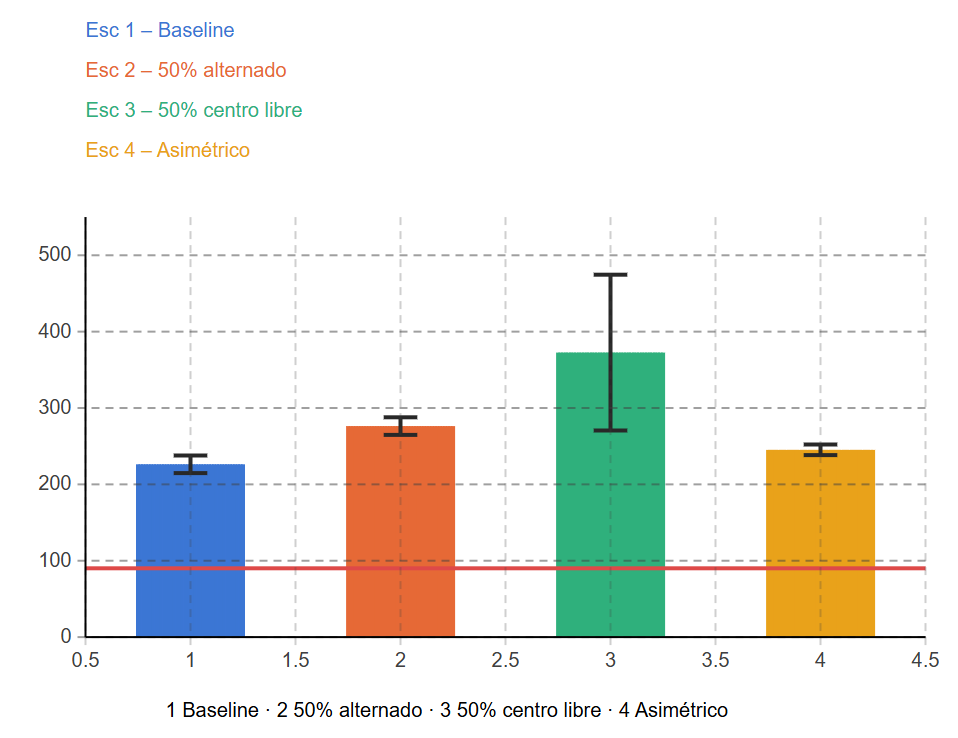
\includegraphics[width=0.75\textwidth]{fig2_barras_ic.png}
    \caption{Tiempo medio de evacuaci\'on por escenario con su intervalo de confianza
    del 95\%. La l\'inea roja marca el umbral de 90 segundos.}
    \label{fig:barras}
\end{figure}

\begin{figure}[H]
\pendiente
    \centering
    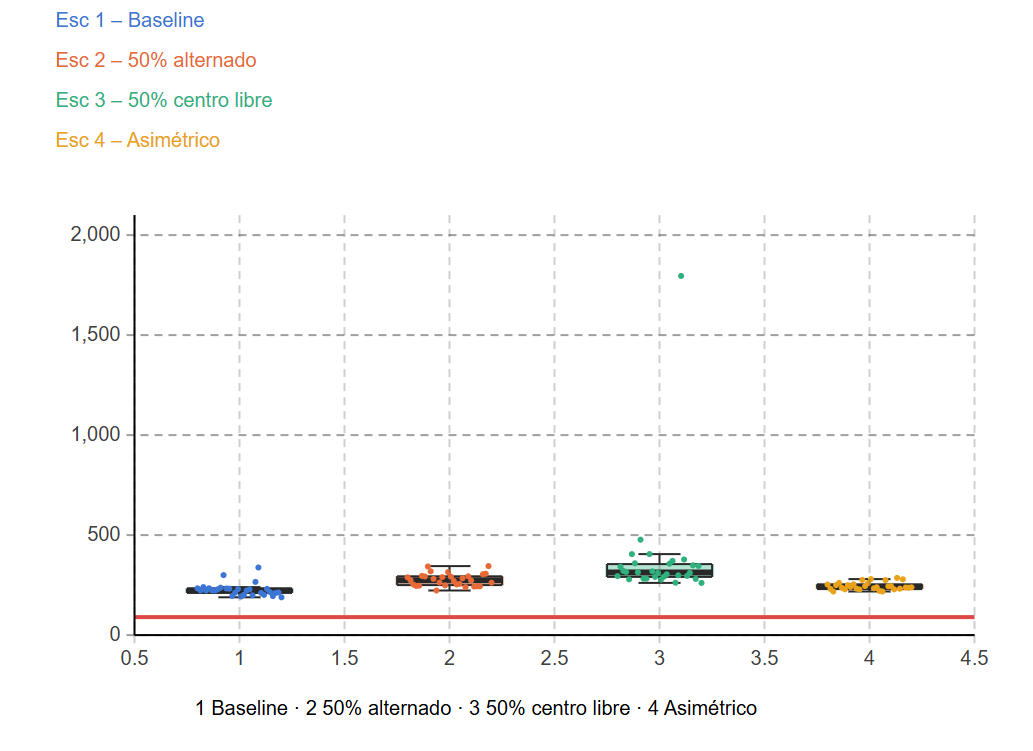
\includegraphics[width=0.8\textwidth]{fig3_boxplot.png}
    \caption{Distribuci\'on de los tiempos de evacuaci\'on de las 30 corridas de cada
    escenario (caja: cuartiles; l\'inea central: mediana; bigotes: 1,5 veces el rango
    intercuart\'ilico; puntos: cada corrida).}
    \label{fig:boxplot}
\end{figure}

\pendiente

Ninguna de las 120 corridas cumple el umbral de 90 segundos, ni siquiera en el
escenario baseline con las seis salidas disponibles (226,2~s en promedio). Esto se
mantiene incluso si se considera solamente el tiempo hasta el \'ultimo pasajero, sin
el tramo final de la tripulaci\'on: 193,0~s en promedio en el baseline.

Con 30 r\'eplicas por escenario las diferencias son estad\'isticamente
significativas (prueba de Mann-Whitney, $p < 0{,}001$ entre escenarios
consecutivos) y permiten ordenar los escenarios de mejor a peor: baseline (mediana
223,4~s), asim\'etrico (240,2~s), 50\% alternado (274,0~s) y 50\% con el centro
libre (313,1~s). El escenario 3 es el m\'as desfavorable: al bloquear las dos salidas
delanteras tipo~I, que la tripulaci\'on abre a los pocos segundos del amerizaje, toda
la evacuaci\'on depende de las salidas sobre el ala, cuya apertura por parte de un
pasajero sin entrenamiento es m\'as lenta.

El escenario 3 incluye adem\'as una corrida at\'ipica de 1.796 segundos, en la que un
grupo de pasajeros qued\'o trabado durante m\'as de 20 minutos antes de evacuar. Se
atribuye a una traba puntual de peatones dentro de la Pedestrian Library y se
declara como limitaci\'on del modelo. Esa sola corrida eleva la media del escenario
de 323,5~s a 372,6~s y ensancha su intervalo de confianza; por ese motivo, para
comparar escenarios se toma como referencia la mediana, que no se ve afectada por
casos aislados.

La diferencia entre el tiempo total y el tiempo de los pasajeros corresponde a la
salida de la tripulaci\'on, que evac\'ua \'ultima: en promedio suma 33,1~s en el
baseline y llega a 62,2~s en el escenario 3.

Resulta llamativo que el escenario asim\'etrico (un lado completo disponible) sea
m\'as r\'apido que el escenario alternado, que es la configuraci\'on t\'ipica de
certificaci\'on, siendo que ambos conservan una salida delantera y dos sobre el ala
en las mismas posiciones a lo largo del fuselaje. Este resultado se interpreta con
cautela y se retoma en las conclusiones.

\subsection{Curva de evacuaci\'on acumulada}

\begin{figure}[H]
\pendiente
    \centering
    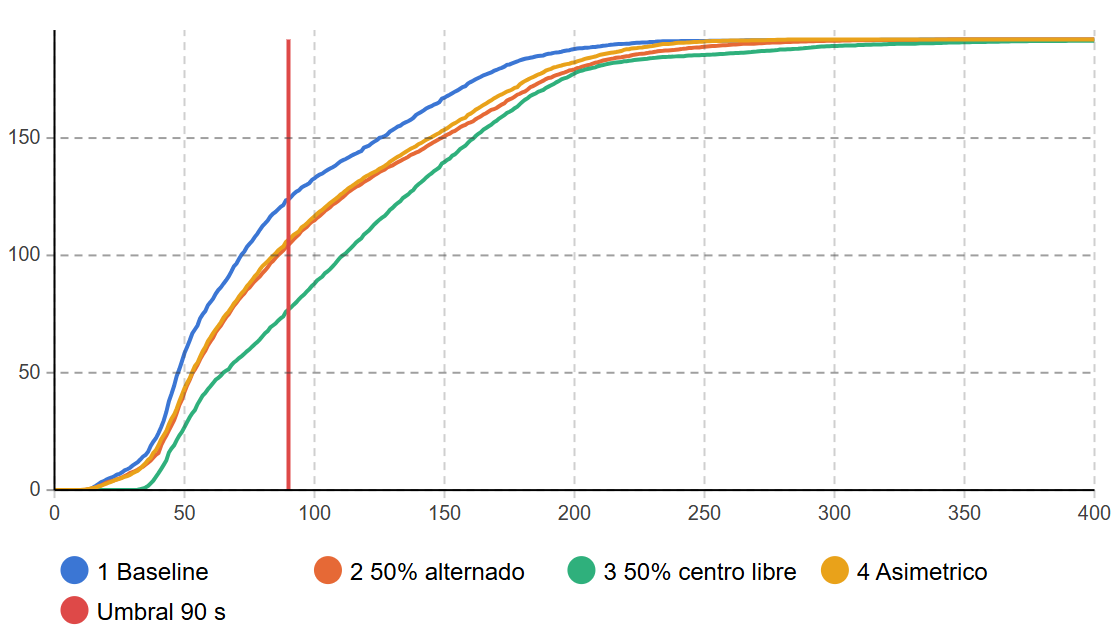
\includegraphics[width=0.85\textwidth]{fig4_curva_acumulada.png}
    \caption{Ocupantes evacuados acumulados en funci\'on del tiempo, promedio de las
    30 corridas de cada escenario. La l\'inea roja vertical marca los 90 segundos.}
    \label{fig:curva}
\end{figure}

\pendiente

Al llegar a los 90 segundos, en promedio evacuaron 124 de los 192 ocupantes en el
baseline (65\%), entre 105 y 107 en los escenarios 2 y 4 (55\%) y 77 en el
escenario 3 (40\%). La curva del escenario 3 adem\'as arranca m\'as tarde: el primer
ocupante sale en promedio a los 38,5~s, contra unos 15~s en el resto de los
escenarios, porque no dispone de las salidas delanteras que abre la tripulaci\'on. En
todos los escenarios la pendiente disminuye en el tramo final, cuando quedan los
pasajeros m\'as alejados de las salidas y la tripulaci\'on.

\subsection{Uso de las salidas}\label{sub:uso_salidas}

\begin{figure}[H]
\pendiente
    \centering
    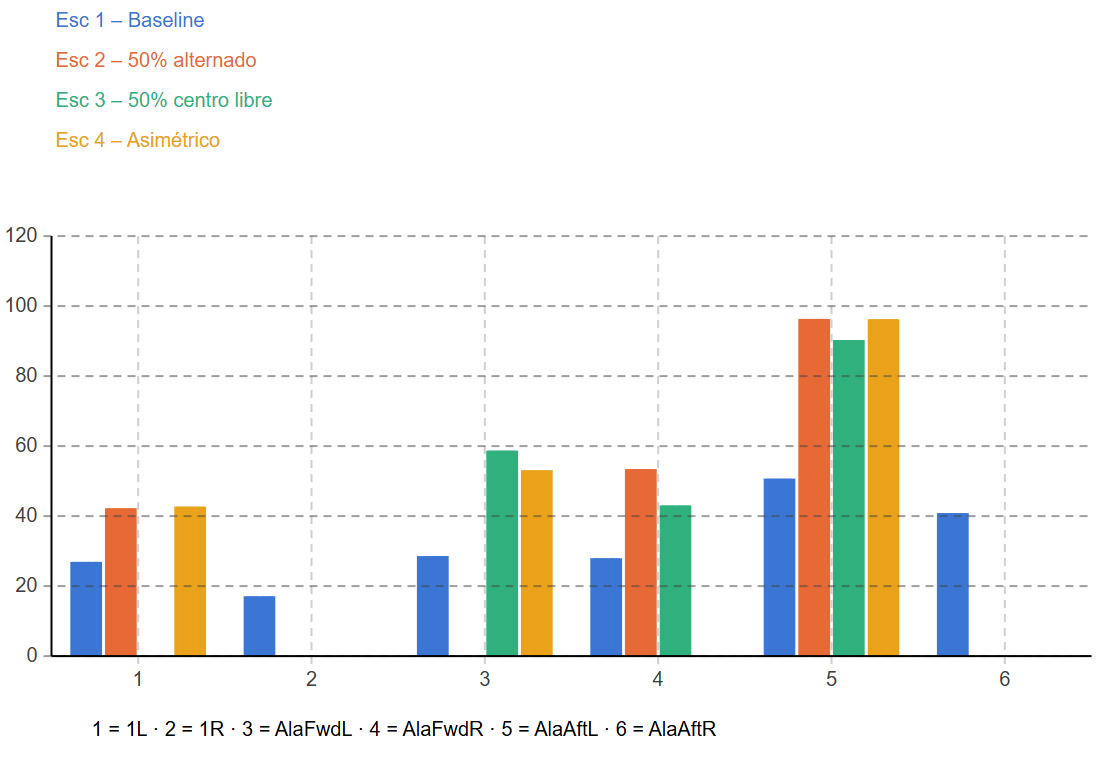
\includegraphics[width=0.85\textwidth]{fig5_uso_salidas.png}
    \caption{Ocupantes evacuados por cada salida (promedio por corrida) en cada
    escenario. Las salidas bloqueadas en un escenario no registran evacuados.}
    \label{fig:uso_salidas}
\end{figure}

\pendiente

La salida sobre el ala trasera izquierda (AlaAftL) es la m\'as utilizada en los
cuatro escenarios: evac\'ua en promedio 51 ocupantes en el baseline y entre 90 y 96
(aproximadamente la mitad del avi\'on) en los escenarios con el 50\% de las salidas
bloqueadas. Se trata del principal cuello de botella del modelo, consecuencia
directa de que las salidas traseras 2L/2R no son utilizables y de que es la salida
m\'as cercana para toda la mitad trasera de la cabina. La concentraci\'on del flujo
en las salidas sobre el ala es coherente con lo observado en el caso Hudson
(secci\'on~\ref{sub:hudson}).

\subsection{Sensibilidad a la cantidad de salidas bloqueadas}\label{sub:res_sens}

\begin{figure}[H]
\pendiente
    \centering
    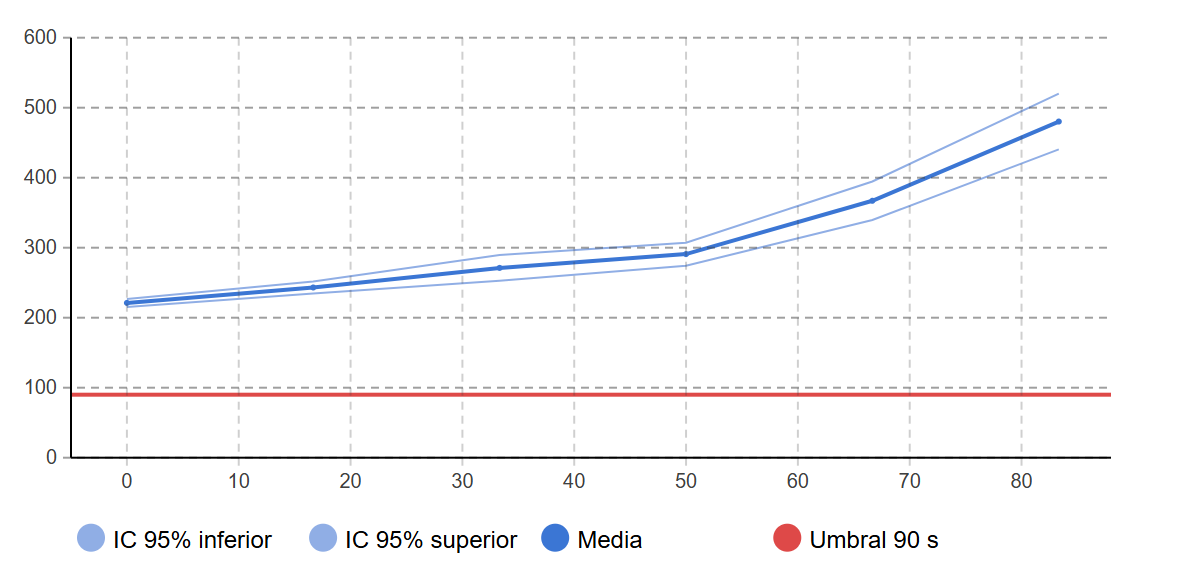
\includegraphics[width=0.85\textwidth]{fig6_sensibilidad.png}
    \caption{Tiempo medio de evacuaci\'on en funci\'on del porcentaje de salidas
    bloqueadas (sobre las 6 utilizables), con su intervalo de confianza del 95\%. La
    l\'inea roja marca el umbral de 90 segundos.}
    \label{fig:sensibilidad}
\end{figure}

\begin{table}[H]
\pendiente
\centering
\small
\begin{tabular}{ccrcrrc}
\toprule
\textbf{Salidas bloqueadas} & \textbf{\% bloqueado} & \textbf{Media (s)} & \textbf{IC 95\% (s)} & \textbf{Mediana (s)} & \textbf{P95 (s)} & \textbf{Corridas completas} \\
\midrule
0 & 0\%  & 221,1 & 215,2 -- 227,0 & 222,2 & 251,5 & 30 / 30 \\
1 & 17\% & 243,2 & 234,6 -- 251,7 & 239,9 & 285,5 & 30 / 30 \\
2 & 33\% & 271,2 & 252,9 -- 289,5 & 262,0 & 365,8 & 30 / 30 \\
3 & 50\% & 290,7 & 274,4 -- 307,1 & 294,5 & 356,7 & 30 / 30 \\
4 & 67\% & 367,0 & 339,5 -- 394,6 & 349,8 & 502,5 & 30 / 30 \\
5 & 83\% & 480,2 & 440,4 -- 520,1 & 436,1 & 643,7 & 30 / 30 \\
\bottomrule
\end{tabular}
\caption{Tiempo total de evacuaci\'on seg\'un la cantidad de salidas bloqueadas, 30
r\'eplicas por nivel.}
\label{tab:sensibilidad}
\end{table}

El tiempo de evacuaci\'on crece de forma sostenida a medida que se pierden salidas,
y el crecimiento se acelera a partir del 50\%: con una sola salida disponible, el
tiempo medio (480,2~s) es m\'as del doble que sin bloqueos (221,1~s). Ning\'un nivel
de bloqueo, incluido el caso sin salidas bloqueadas, se acerca al umbral de 90
segundos. Con cinco salidas bloqueadas importa adem\'as cu\'al es la que queda
disponible: cuando la \'unica salida es la delantera derecha (1R), el tiempo medio
ronda los 677~s, contra unos 415~s cuando es una de las salidas traseras sobre el
ala, aunque con 3 a 6 corridas por caso esa diferencia es solo indicativa.

Todas las corridas de este experimento terminaron, pero en algunos niveles aparecen
corridas notablemente m\'as largas que el resto (por ejemplo, 832~s con cinco salidas
bloqueadas o 642~s con cuatro), que elevan la media por encima de la mediana. Como en
el experimento anterior, se atribuyen a trabas puntuales de peatones y se declaran
como limitaci\'on del modelo.

Como verificaci\'on cruzada, el caso sin salidas bloqueadas de este experimento
(221,1~s) no presenta diferencias significativas con el escenario baseline del
experimento anterior (226,2~s; prueba de Mann-Whitney, $p = 0{,}71$), aunque ambos
resultados se generan por caminos distintos del modelo.

% =============================================================================
\newpage
\section{Conclusiones}
% =============================================================================

\subsection{Respuesta a la pregunta central}

\pendiente

La pregunta que gui\'o este trabajo era en qu\'e medida el cumplimiento de la regla
de los 90 segundos se sostiene cuando las condiciones de evacuaci\'on dejan de ser
las estandarizadas del ensayo de certificaci\'on. Bajo las condiciones modeladas, la
respuesta es que no se sostiene en ninguna de las configuraciones analizadas:
ninguna de las 300 corridas realizadas, entre los dos experimentos, evacu\'o a los
192 ocupantes en 90 segundos o menos.

La distancia respecto del umbral no es marginal. Aun en el escenario m\'as favorable,
con las seis salidas utilizables disponibles, el tiempo mediano de evacuaci\'on fue
de 223,4 segundos, unas 2,5 veces el umbral normativo, y a los 90 segundos hab\'ia
evacuado en promedio alrededor del 65\% de los ocupantes. Tampoco se alcanza el
umbral si se descuenta la salida de la tripulaci\'on: el \'ultimo pasajero abandon\'o
el avi\'on, en promedio, a los 193 segundos.

\subsection{Factores que m\'as inciden en el tiempo de evacuaci\'on}

\pendiente

\textbf{Disponibilidad y ubicaci\'on de las salidas.} La p\'erdida de salidas es el
factor con mayor efecto: el tiempo crece de forma sostenida a medida que se bloquean
salidas y el crecimiento se acelera a partir del 50\%, hasta duplicarse cuando queda
una sola salida. Pero no alcanza con saber cu\'antas salidas se pierden, sino
cu\'ales: los tres escenarios que bloquean el 50\% de las salidas dieron tiempos
medianos de entre 240 y 313 segundos. El caso m\'as desfavorable fue el que bloquea
las dos salidas delanteras, porque son las que abre la tripulaci\'on entrenada a los
pocos segundos del amerizaje; sin ellas, toda la evacuaci\'on depende de salidas que
deben abrir pasajeros sin entrenamiento.

\textbf{Concentraci\'on del flujo sobre el ala.} Al quedar inutilizadas las salidas
traseras, la salida sobre el ala trasera izquierda pasa a ser la m\'as cercana para
toda la mitad posterior de la cabina y se convierte en el principal cuello de botella
del modelo: en los escenarios con el 50\% de las salidas bloqueadas, por ella
evac\'ua aproximadamente la mitad de los ocupantes. La actitud de cola baja propia
del amerizaje, que inutiliza las salidas traseras, condiciona as\'i el desempe\~no de
todas las configuraciones.

\textbf{Salida de la tripulaci\'on en \'ultimo lugar.} El procedimiento por el cual
la tripulaci\'on evac\'ua despu\'es del \'ultimo pasajero agrega entre 33 y 62
segundos al tiempo total seg\'un el escenario. Este tramo, que la norma incluye en la
medici\'on al contar a todos los ocupantes, por s\'i solo representa entre un tercio
y dos tercios del umbral de 90 segundos.

\subsection{Configuraci\'on alternada frente a configuraci\'on asim\'etrica}

\pendiente

Un resultado que no se anticipaba es que el escenario con un lado completo
disponible (asim\'etrico) result\'o m\'as r\'apido que el escenario alternado, que
es la distribuci\'on de salidas bloqueadas t\'ipica del ensayo de certificaci\'on:
240,2~s contra 274,0~s de mediana, con una diferencia estad\'isticamente
significativa. Ambos conservan una salida delantera y dos sobre el ala en las mismas
posiciones a lo largo del fuselaje, por lo que la diferencia no se explica por la
distancia a recorrer.

Una explicaci\'on posible, que el modelo no permite confirmar, es la direcci\'on de
los cruces del pasillo. En ambos casos los pasajeros desconocen qu\'e salidas est\'an
bloqueadas y algunos deben cruzar al otro lado de la cabina al encontrar cerrada la
salida que eligieron. En el escenario asim\'etrico todos esos cruces ocurren en el
mismo sentido, mientras que en el alternado se producen en sentidos opuestos en la
zona de las salidas sobre el ala (hacia la derecha en la salida delantera y hacia la
izquierda en la trasera), lo que genera flujos encontrados en un pasillo que solo
admite dos personas en paralelo. M\'as all\'a de su causa, el resultado sugiere que
la configuraci\'on utilizada en la certificaci\'on no es necesariamente la m\'as
exigente ni la m\'as representativa de un evento real.

\subsection{Implicancias para la norma}

\pendiente

Los resultados no permiten afirmar que el Boeing 737-800 no cumpla con la
certificaci\'on vigente: el modelo no reproduce el ensayo normativo, sino que lo
somete deliberadamente a condiciones m\'as exigentes. Lo que s\'i muestran es que,
cuando a la configuraci\'on de salidas se le suman el equipaje de mano, los pasajeros
con movilidad reducida, la iluminaci\'on de emergencia, el desconocimiento de las
salidas bloqueadas, la apertura de las salidas por parte de pasajeros sin
entrenamiento y la evacuaci\'on final de la tripulaci\'on, el tiempo de evacuaci\'on
se aleja sistem\'aticamente del umbral de 90 segundos, y lo hace en todas las
configuraciones evaluadas.

A partir de estos resultados, el equipo considera que este escenario podr\'ia
ponerse a disposici\'on de los organismos certificadores (FAA y EASA) como insumo
para su an\'alisis. Corresponde a ellos evaluar si las condiciones incorporadas son
representativas de un evento real y, en ese caso, decidir si mantener el umbral de
90 segundos, ampliarlo para estas condiciones, o requerir que las aeronaves vuelvan
a demostrar su cumplimiento bajo un ensayo m\'as realista.

\subsection{Limitaciones}

Estas conclusiones deben leerse a la luz de las limitaciones del modelo:

\textbf{Estimaci\'on conservadora.} La comparaci\'on con el caso Hudson (secci\'on
~\ref{sub:hudson}) mostr\'o que el modelo asume una apertura de las salidas sobre el ala m\'as
lenta que la observada, no representa a la tripulaci\'on guiando a los pasajeros
hacia las salidas delanteras y no permite el paso entre filas de asientos. Las tres
simplificaciones tienden a aumentar el tiempo de evacuaci\'on, por lo que los valores
obtenidos deben interpretarse como una cota superior m\'as que como una predicci\'on
exacta.

\textbf{Par\'ametros de calibraci\'on propios.} El di\'ametro efectivo de los
pasajeros, el ancho de pasillo modelado y los tiempos de apertura de las salidas son
supuestos del equipo, justificados en las secciones~\ref{sub:poblacion} y~\ref{sub:logica}, y no valores medidos.
Distintos valores razonables podr\'ian desplazar los tiempos obtenidos.

\textbf{Trabas puntuales de peatones.} En un peque\~no n\'umero de corridas, grupos
de pasajeros quedaron detenidos durante un tiempo prolongado por limitaciones de la
Pedestrian Library de AnyLogic. Estos casos se conservaron en los datos y se mitig\'o
su efecto informando la mediana junto con la media.

\textbf{Validaci\'on cualitativa.} El \'unico amerizaje comercial documentado en
detalle no registra un tiempo total de egreso comparable, por lo que la validaci\'on
contra el caso real se limit\'o a los patrones de evacuaci\'on y no a los tiempos.

% =============================================================================
\newpage
\section{Material complementario}
% =============================================================================

\subsection{Modelo publicado en AnyLogic Cloud}

El modelo completo, con sus tres experimentos (Simulation, Escenarios y
Sensibilidad), se encuentra publicado en AnyLogic Cloud y puede ejecutarse desde
el navegador sin necesidad de instalar AnyLogic:

\url{https://cloud.anylogic.com/model/03124131-1043-4190-adb5-7e8a0695af43}


\begin{table}[H]
\centering
\small
\begin{tabular}{lll}
\toprule
\textbf{Integrante} & \textbf{Legajo} & \textbf{Correo electr\'onico} \\
\midrule
Luis Parmigiani   & 52933 & \texttt{parmigianiluis04@gmail.com} \\
Agust\'in Dana    & 52935 & \texttt{agusidana04@gmail.com} \\
Bruno Vitali      & 53137 & \texttt{brunoVitali33@gmail.com} \\
St\'efano Conti   & 52850 & \texttt{stefano.conti2004@gmail.com} \\
\bottomrule
\end{tabular}
\caption{Integrantes del equipo y datos de contacto.}
\label{tab:integrantes}
\end{table}

\subsection{Video de demostraci\'on}

El siguiente video muestra una corrida del modelo con animaci\'on de los agentes y
la ejecuci\'on de los experimentos utilizados para obtener los resultados de la
secci\'on~\ref{sec:resultados}:

\completar{LINK AL VIDEO DE DEMOSTRACI\'ON EN YOUTUBE}

% =============================================================================
\newpage
\nocite{anylogic2023}
\bibliographystyle{unsrt}
\bibliography{referencias}

\end{document}
